\paragraph{Question and comparable evidence.}
The terrain branch asks whether fitted map-conditioned corrections improve
on its history-only base, not whether ordinary HSM-SDE beats CV. All ten
configurations were fitted and forecasts were executed. The original primary
grid contains 2,300 distinct slots: 2,297 successful and three failed, with
no pending or missing slots. To compare the same observations, we describe
the intersection of 43 recording blocks for which all ten configurations
have all five successful seed forecasts (2,150 slots). Three entire blocks
are excluded from this post-hoc comparison; no failed result is set to zero
or replaced. Selection uses execution status, not which model wins, but
still conditions on successful execution. These summaries do not estimate
performance on the original full 46-block population or replace its
registered inference. Seeds are averaged within a block before blocks
receive equal weight. All underlying scores and forecasts are unchanged.

\paragraph{Overall combination: no descriptive aggregate gain.}
The current all-terrain configuration is worse than its history base on
both average ES and thirty-minute mean-position error. In this implementation,
simply adding every terrain feature has not produced an average gain.
On this common subset, all-terrain has average ES 482.06 m versus 455.08 m
for base, a change of $+26.98$ m, and FDE 1459.37 versus 1420.37 m,
a change of $+39.00$ m (Table~\ref{tab:terrain-description}). Its ES is
higher at all four targets; the 30-minute difference is $+69.11$ m
(Figure~\ref{fig:terrain-description}). Yet all-terrain has lower average
ES in 22 of the 43 individual blocks. Thus the aggregate disadvantage
coexists with heterogeneous local gains; selected successful case maps
cannot establish an average terrain benefit. This is a descriptive result
about this fitted combination on the selected subset, not a significant
harm verdict or proof that terrain information is intrinsically unhelpful.

\begin{table}[!htbp]\centering
\caption{Terrain predictions on the same 43 complete recording blocks (five seeds each). ES averages four targets; $\Delta$ES is relative to base. FDE, coverage and area use 30 minutes. Success counts retain all 230 original slots per configuration. These are post-hoc descriptive means, not the registered full-family effects.}\label{tab:terrain-description}
\small\setlength{\tabcolsep}{3pt}
\begin{tabular}{lrrrrrr}\toprule
Configuration & ES (m) & $\Delta$ES (m) & FDE (m) & Cover (\%) & Area (km$^2$) & Success\\\midrule
base & 455.08 & +0.00 & 1420.37 & 46.05 & 5.503 & 230/230\\
all-terrain & 482.06 & +26.98 & 1459.37 & 40.47 & 5.609 & 229/230\\
lio-road & 498.04 & +42.96 & 1493.33 & 52.09 & 6.202 & 229/230\\
lio-river & 455.27 & +0.19 & 1478.38 & 41.40 & 5.701 & 229/230\\
lio-worldcover & 453.44 & -1.64 & 1414.40 & 49.77 & 5.635 & 230/230\\
lio-surface & 462.66 & +7.58 & 1410.27 & 47.44 & 5.670 & 230/230\\
loo-road & 462.19 & +7.11 & 1459.69 & 44.65 & 5.719 & 230/230\\
loo-river & 498.29 & +43.20 & 1446.22 & 50.23 & 5.693 & 230/230\\
loo-worldcover & 482.14 & +27.06 & 1465.55 & 41.40 & 5.886 & 230/230\\
loo-surface & 477.11 & +22.03 & 1485.96 & 46.51 & 6.145 & 230/230\\
\bottomrule\end{tabular}
\end{table}

\begin{figure}[!htbp]\centering
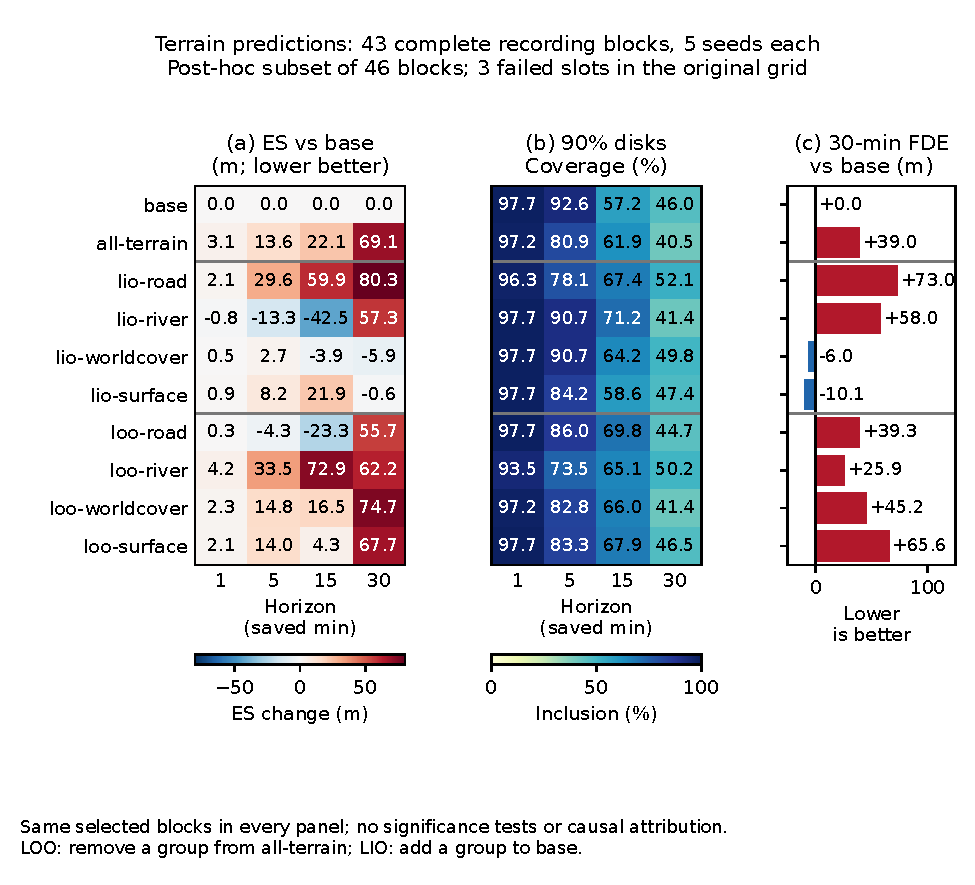
\includegraphics[width=\linewidth]{../figures/terrain-description-v1/terrain-evidence.pdf}
\caption{Existing terrain forecasts on the same post-hoc 43-block subset.
Left: four horizon-specific ES differences from history-only base; negative
is favourable. Middle: actual inclusion in nominal 90\% disks, with 90\%
as the calibration target. Right: 30-minute predictive-mean error differences
from base. All panels use identical blocks and equal five-seed/block
weighting. LIO adds one group to base; LOO removes a group and dependent
interactions from all-terrain. Panels compare configuration performance,
not isolated factor effects. Missingness in the full grid is retained in
Table~\ref{tab:terrain-description}; no inferential intervals are supplied.}
\label{fig:terrain-description}\end{figure}

\paragraph{Factor configurations: context and horizon matter.}
Adding the current road features accompanies worse scores; removing them
improves scores in the compared configurations.
Adding the road group alone increases average ES by 42.96 m relative to
base; removing it from all-terrain decreases ES by 19.87 m. Both directions
associate the current road representation with a score cost in these fitted
configurations, not a general claim that roads cannot help prediction.
The river-only configuration's benefit does not carry from 15 to 30 minutes:
improvement at a shorter horizon does not imply improvement farther ahead.
It reduces 15-minute ES by 42.51 m but increases
30-minute ES by 57.27 m relative to base. Its average ES change is only
$+0.19$ m, whereas removing river from the full combination increases
average ES by 16.22 m. A factor's standalone result therefore does not
determine its role in the full configuration.

Adding land cover alone lowers average ES by 1.64 m and final mean-position
error by 5.96 m, showing a small favourable mean result. Its average ES is
453.44 m, the lowest of these ten saved configuration means, not a confirmed
general advantage. Surface-only instead increases average ES by 7.58 m while
lowering FDE by 10.09 m. These illustrate a small favourable configuration
and a score--location trade-off, respectively, not confirmed factor
superiority. Fits, diffusion, interactions and effective regularisation
change across configurations, so these differences cannot be assigned to
isolated causal terrain effects.

\paragraph{Larger paired subsets and prediction-region limits.}
As a descriptive sensitivity check, each candidate/control pair can retain
all of its five-seed-complete blocks: 45 for comparisons involving a failed
configuration, 46 for complete single-group/base pairs. All-terrain/base
then changes ES by $+21.17$ m; road-only/base by $+41.18$ m; removing road
by $-18.50$ m; and land-cover-only/base by $-3.81$ m. Those directions agree
with the common-subset summaries. River-only/base changes from $+0.19$ to
$-1.54$ m, showing the fragility of its near-zero average. The larger subsets
also condition on success, use different blocks and cannot repair the
missing full-cohort estimand or justify a global ranking.

Thirty-minute nominal 90\% coverage spans only 40.47--52.09\% across the ten
configurations on the common subset. All-terrain covers 40.47\% versus
base's 46.05\%, despite slightly greater mean area, 5.609 versus 5.503
km$^2$. Terrain conditioning has therefore not made the long-horizon disks
empirically reliable in this comparison. Taken together, the saved data
show configuration-dependent and horizon-dependent trade-offs, not a
uniform gain from adding every terrain group. The registered full-family
answer remains separately unavailable under the original rule below.
